\chapter{自旋与极化的进一步讨论 (More on Spin and Polarization)}\label{ch:morespin}

本章在第~\ref{ch:spin2p}~章关于带自旋的两粒子散射的基础上，进一步深入讨论自旋自由度的处理方法与极化测量。先以密度矩阵的语言一般地刻画极化态与混合态，再以 (Spin~$1/2$)–(Spin~$0$) 弹性散射作为重要范例，说明如何通过测量微分截面的非对称性来抽取入射极化与散射振幅信息。最后引入螺旋度 (helicity) 表示，给出两粒子态的螺旋度基矢、$S$ 矩阵元、分波展开和 Wigner $D$ 函数所满足的若干关系，为相对论性散射的处理铺垫基础。本章的主要参考为 Taylor《Scattering Theory》中关于自旋与螺旋度形式的章节。

\section{极化态与密度矩阵 (Polarization and Density Matrix)}

\subsection{为何引入密度矩阵}

利用极化粒子作散射可以得到比无极化情形更多的散射振幅信息。然而，实验上往往很难得到完全极化的入射粒子束或靶粒子：
\begin{itemize}
  \item 在外磁场中，粒子沿磁场方向极化的粒子数遵从 Boltzmann 分布
  \[
    \propto \exp\!\left(\frac{m\mu B}{kT}\right),
  \]
  这通常给出仅有部分极化的束流。
  \item 加速器或自然来源（例如 $\beta$ 衰变）给出的粒子束可能并不极化，或仅沿动量方向极化。
\end{itemize}
因此一般情形下，描述粒子的自旋状态需要使用 \emph{密度矩阵 (density matrix)}，而非单一的纯态矢量。

\subsection{纯态、混合态与密度矩阵}

对量子系统的状态作如下区分：
\begin{definition}[纯态与混合态]
\label{def:pure-mixed}
设 $\Hilb$ 为系统的 Hilbert 空间。
\begin{itemize}
  \item \emph{纯态 (pure state)}：可由单一态矢量 $\ket{\psi}\in\Hilb$ 描述。
  \item \emph{混合态 (mixed state)}：系统以概率 $w_i$ 处于纯态 $\ket{\psi^i}$。其 Hermite 密度算符 (density matrix) 定义为
  \begin{equation}
    \rho \;=\; \sum_i w_i \,\ket{\psi^i}\bra{\psi^i}, \qquad \sum_i w_i = 1, \quad w_i\geq 0.
    \label{eq:rho-def}
  \end{equation}
\end{itemize}
\end{definition}

任意力学量算符 $\Op{A}$ 在状态 $\rho$ 下的平均值为
\begin{equation}
  \expval{A}_\rho \;=\; \Tr(\Op{A}\rho) \;=\; \sum_i w_i \matel{\psi^i}{\Op{A}}{\psi^i}.
  \label{eq:rho-avg}
\end{equation}

对于纯态 $\rho=\ket{\psi}\bra{\psi}$，有 $\rho^2=\rho$；一般而言 $\Tr\rho=1$。为方便起见也允许放松归一化条件，此时
\begin{equation}
  \expval{A}_\rho \;=\; \frac{\Tr(\Op{A}\rho)}{\Tr\rho}.
  \label{eq:rho-avg-normalized}
\end{equation}

\subsection{自旋部分的密度矩阵}

考虑自旋为 $s$ 的粒子系统，仅看自旋自由度，密度矩阵 $\rho$ 是 $(2s+1)\times(2s+1)$ 矩阵。其分类如下：
\begin{itemize}
  \item \emph{完全极化 (completely polarized)}：$\rho=\ket{\chi}\bra{\chi}$，$\rho^2=\rho$；这是纯态。
  \item \emph{完全非极化 (completely unpolarized)}：
  \begin{equation}
    \rho \;=\; \sum_m \frac{1}{2s+1}\,\ket{m}\bra{m} \;=\; \frac{1}{2s+1}\, I,
    \label{eq:unpolarized}
  \end{equation}
  与所选取的基矢无关。从物理上说，它等价于：
  \begin{itemize}
    \item 极化方向完全随机；
    \item 处于各种不同极化方向的概率相同；
    \item 在任何转动操作下，系统的任何观测量的平均值结果不变（参见 Schur 引理）。
  \end{itemize}
  \item \emph{部分极化 (partial polarization)}：介于上述两者之间。
\end{itemize}

\subsection{自旋 $1/2$ 情形：极化矢量}

对于自旋 $1/2$ 的态，$\rho$ 是 $2\times 2$ Hermite 矩阵，可一般地写成
\begin{equation}
  \rho \;=\; \lambda\,(1+\bm{\pi}\cdot\bm{\sigma}), \qquad \lambda\in\R,\quad \bm{\pi}\in\R^3.
  \label{eq:spinhalf-rho}
\end{equation}
取 $\Tr\rho=2\lambda=1$，即 $\lambda=1/2$。称 $\bm{\pi}$ 为 \emph{极化矢量 (polarization vector)}。

\begin{proposition}[$\bm{\pi}$ 的物理意义]
\label{prop:pi-meaning}
对于密度矩阵 $\rho=\tfrac{1}{2}(1+\bm{\pi}\cdot\bm{\sigma})$，
\begin{enumerate}
  \item $\bm{\pi}=\expval{\bm{\sigma}}_\rho$，并满足 $0\leq |\bm{\pi}|\leq 1$；
  \item 若 $|\bm{\pi}|=1$，$\rho$ 代表完全极化的纯态，即 $\bm{\pi}\cdot\bm{s}$ 的本征态；
  \item 若 $\bm{\pi}=0$，则代表完全非极化的态；
  \item 若 $0<|\bm{\pi}|<1$，则代表部分极化。
\end{enumerate}
\end{proposition}

也即 $\bm{\pi}$ 可以作为一个代表量来描述自旋态。对两粒子态 $s_1,s_2$，一般密度矩阵是 $(2s_1+1)(2s_2+1)$ 维矩阵。

\subsection{含空间自由度的密度矩阵}

考虑到粒子的空间自由度：若空间运动处于纯态 $\ket{\phi}\in\Hilb_{\text{space}}$，自旋处于混合态、密度矩阵 $\rho$ 作用在 $\Hilb_{\text{spin}}$ 上，则总密度算符为
\begin{equation}
  \rho_{\text{total}} \;=\; \big(\ket{\phi}\bra{\phi}\big)\otimes \rho.
  \label{eq:total-rho}
\end{equation}
也可以采用混合的表示方式：空间部分用 $\ket{\phi}$，自旋部分用 $\rho$。例如后面我们关心的两粒子态，空间部分用 $\ket{\bm p_1,\bm p_2}$，自旋部分用 $\rho$。

\section{入射、出射密度矩阵与极化散射截面}
\label{sec:inout-density}

考虑散射过程
\[
  (\bm{p},\chi_{\text{in}}) \to (\bm{p}',\chi_{\text{out}}),
\]
散射振幅算符 $F$（作用在自旋空间）将入射自旋态映为出射自旋态：
\begin{equation}
  \chi_{\text{out}} \;=\; F(\bm{p}'\!\leftarrow\bm{p})\,\chi_{\text{in}}.
  \label{eq:F-action}
\end{equation}
若 $\|\chi_{\text{in}}\|=1$，则 $\|\chi_{\text{out}}\|^2$ 即为末态中处于 $\bm{p}'$ 方向的概率分布，对应微分散射截面。

\subsection{出射密度矩阵的计算}

若入射自旋态是混合态，
\[
  \rho_{\text{in}} \;=\; \sum_i w_i\,\ket{\chi_{\text{in}}^i}\bra{\chi_{\text{in}}^i},
\]
则出射自旋部分密度矩阵为
\begin{align}
  \rho_{\text{out}}
  &=\sum_i w_i\,\ket{\chi_{\text{out}}^i}\bra{\chi_{\text{out}}^i}
   = \sum_i w_i\, F\,\ket{\chi_{\text{in}}^i}\bra{\chi_{\text{in}}^i}\,F^\dagger \notag\\
  &= F(\bm{p}'\!\leftarrow\bm{p})\,\rho_{\text{in}}\,F^\dagger(\bm{p}'\!\leftarrow\bm{p}).
  \label{eq:rhoout}
\end{align}

由于
\[
  \frac{\rmd\sigma}{\rmd\Omega}(\bm{p}'\!\leftarrow\bm{p},\chi^i_{\text{in}})
  \;=\; \|\chi_{\text{out}}^i\|^2,
\]
对入射混合态求平均得到末态极化求和后的微分截面：
\begin{align}
  \Tr[\rho_{\text{out}}]
  &= \sum_i w_i\,\|\chi_{\text{out}}^i\|^2
   = \sum_i w_i\,\frac{\rmd\sigma}{\rmd\Omega}(\bm{p}'\!\leftarrow\bm{p},\chi^i_{\text{in}}) \notag\\
  &\equiv \frac{\rmd\sigma}{\rmd\Omega}(\bm{p}'\!\leftarrow\bm{p},\rho_{\text{in}}).
  \label{eq:dsigma-rho-spinhalf}
\end{align}
这就是对入射态不同极化求平均、末态极化求和后的微分截面，可直接用 $\rho_{\text{in}}$ 表示。

\section{(Spin $1/2$)–(Spin $0$) 散射的极化分析}
\label{sec:half-zero-scattering}

我们利用上述形式讨论 (Spin~$1/2$)–(Spin~$0$) 弹性散射。$\rho_{\text{in}},\rho_{\text{out}}$ 可以用 $\bm{\pi}_{\text{in,out}}$ 表示；$\rho_{\text{in}}$ 已归一化，
\begin{equation}
  \rho_{\text{in}} \;=\; \tfrac{1}{2}\,[1+\bm{\pi}_{\text{in}}\cdot\bm{\sigma}].
  \label{eq:rhoin-piin}
\end{equation}

\subsection{由对称性导出的振幅形式}

若系统满足转动对称性以及空间反射 (P) 对称性，则散射振幅在自旋空间中只能取如下形式（参见第~\ref{ch:invariance}~章中关于不变性原理的讨论）：
\begin{equation}
  F(\bm{p}'\!\leftarrow\bm{p}) \;=\; a(\theta)\,I + \rmi\, b(\theta)\,\hat{\bm{n}}\cdot\bm{\sigma}, \qquad \hat{\bm{n}} = \frac{\bm{p}\times\bm{p}'}{|\bm{p}\times\bm{p}'|}.
  \label{eq:F-rotpar}
\end{equation}
$\hat{\bm n}$ 选作散射平面的法向；$a(\theta), b(\theta)$ 是仅依赖极角的复函数。

\subsection{出射密度矩阵与极化}

将~\eqref{eq:F-rotpar}~代入~\eqref{eq:rhoout}：
\begin{align}
  \rho_{\text{out}}
  &= F(\bm{p}'\!\leftarrow\bm{p})\,\rho_{\text{in}}\,F^\dagger(\bm{p}'\!\leftarrow\bm{p}) \notag\\
  &= \tfrac{1}{2}\big(a(\theta)I + \rmi b(\theta)\hat{\bm n}\cdot\bm{\sigma}\big)
     [1+\bm{\pi}_{\text{in}}\cdot\bm{\sigma}]
     \big(a^*(\theta)I - \rmi b^*(\theta)\hat{\bm n}\cdot\bm{\sigma}\big) \notag\\
  &= \tfrac{1}{2}\big(|a|^2 + |b|^2 + 2\,\mathrm{Im}(ab^*)\,\hat{\bm n}\cdot\bm{\pi}_{\text{in}}\big)
     \big[1 + \bm{\pi}_{\text{out}}\cdot\bm{\sigma}\big].
  \label{eq:rho-out-spinhalf}
\end{align}
具体的 $\bm{\pi}_{\text{out}}$ 形式将在后文按需要给出（先不写出）。

\subsection{末态极化求和的微分截面}

末态极化不分辨即对极化求和，由~\eqref{eq:dsigma-rho-spinhalf}~得
\begin{align}
  \frac{\rmd\sigma}{\rmd\Omega}(\bm{p}'\!\leftarrow\bm{p},\bm{\pi}_{\text{in}})
  &= \Tr[\rho_{\text{out}}] = |a(\theta)|^2 + |b(\theta)|^2 + 2\,\mathrm{Im}(ab^*)\,\hat{\bm n}\cdot\bm{\pi}_{\text{in}} \notag\\
  &= \big[\,|a(\theta)|^2 + |b(\theta)|^2\,\big]\,\big[1 + \nu(\theta)\,\hat{\bm n}\cdot\bm{\pi}_{\text{in}}\big],
  \label{eq:dsigma-piin}
\end{align}
其中
\begin{equation}
  \nu(\theta) \;=\; \frac{2\,\mathrm{Im}(ab^*)}{|a(\theta)|^2 + |b(\theta)|^2}.
  \label{eq:nu-def}
\end{equation}

\paragraph{特殊情况：完全无极化入射} 若 $\bm{\pi}_{\text{in}}=0$，则
\begin{equation}
  \frac{\rmd\sigma}{\rmd\Omega}(\bm{p}'\!\leftarrow\bm{p},\bm{\pi}_{\text{in}}=0)
  \;=\; |a(\theta)|^2 + |b(\theta)|^2.
  \label{eq:dsigma-unpol}
\end{equation}

\paragraph{有极化入射}
若 $\bm{\pi}_{\text{in}}\neq 0$，选 $\bm{\pi}_{\text{in}}$ 在 $y$–$z$ 平面内、与 $z$ 轴的极角为 $\alpha$，散射在通常的极坐标 $\varphi$ 方位角下进行；则
\begin{equation}
  \nu(\theta)\,\hat{\bm n}\cdot\bm{\pi}_{\text{in}}
  \;=\; \nu(\theta)\,|\bm{\pi}_{\text{in}}|\,\sin\alpha\,\cos\varphi.
  \label{eq:nu-n-pi}
\end{equation}
若我们已知 $a,b$（即知道 $F$），通过测量两个不同方位角下的微分截面就能得到 $\hat{\bm n}\cdot\bm{\pi}_{\text{in}}$，再结合 $\alpha$ 已知，可定出 $\bm{\pi}_{\text{in}}$。

\section{典型的极化测量实验}

\subsection{电子–原子核散射：测量入射极化}

假设散射振幅可以理论计算（即 $a,b$ 已知），我们可以通过测量散射截面来反推 $\bm{\pi}_{\text{in}}$ —— 在相对论性的散射理论中，类似的结论也适用。设想如下实验布置：
\begin{itemize}
  \item 由 $\beta$ 衰变得到的电子，初始极化与动量平行，即 $\hat{\bm n}\cdot\bm{\pi}_{\text{in}}=0$（因 $\hat{\bm n}\perp\bm p$），前面的讨论无法直接用；
  \item 用电场改变电子的动量方向，转动 $90^\circ$。这样可选定极化方向为 $\hat{\bm 2}$，新动量方向为 $\hat{\bm 3}$；
  \item 金箔放在电子的路径上，位于 $x$–$y$ 平面上；两个探测器布置在 $x$–$z$ 平面上，对称地分置于左右两侧。
\end{itemize}

设 $n$ 为入射电子数乘以单位面积金箔上原子数。则两侧探测器记录的事件数分别为
\[
  N_{L,R} \;=\; n\,\rmd\Omega\,\big(|a|^2+|b|^2\big)\,\big(1 + \nu\,\hat{\bm n}_{L,R}\cdot\bm{\pi}_{\text{in}}\big),
\]
其中两个探测器对应的法向相反，$\hat{\bm n}_L=-\hat{\bm n}_R=\hat{\bm 2}$（$\hat{\bm n}=\bm p\times\bm p'$）。定义不对称参数
\begin{equation}
  \epsilon \;\equiv\; \frac{N_L - N_R}{N_L + N_R} \;=\; \nu(\theta)\,\hat{\bm 2}\cdot\bm{\pi}_{\text{in}}.
  \label{eq:asym}
\end{equation}
测量 $\epsilon$ 即可定出 $\bm{\pi}_{\text{in}}$。

\subsection{质子–无自旋核散射：双散射法测量振幅}
\label{subsec:double-scattering}

例：振幅 $F$ 未知，希望用数据来获取 $F$ 的信息（如质子与无自旋原子核散射）。
\begin{itemize}
  \item 加速器发出的质子通常没有被极化；散射只能给出 $|a|^2 + |b|^2$ 的信息（参见~\eqref{eq:dsigma-unpol}）。
  \item 即使初始粒子束是非极化的，碰撞之后会变成有极化的。
\end{itemize}
对于 $\bm{\pi}_{\text{in}}=0$，
\begin{align}
  \rho_{\text{out}} &= F\,\rho_{\text{in}}\,F^\dagger
  \;=\; \tfrac{1}{2}\,\big(a + \rmi b\,\hat{\bm n}\cdot\bm{\sigma}\big)\big(a^* - \rmi b^*\,\hat{\bm n}\cdot\bm{\sigma}\big) \notag\\
  &= \tfrac{1}{2}\big(|a|^2 + |b|^2\big)\,\big[1 + \nu(\theta)\,\hat{\bm n}\cdot\bm{\sigma}\big],
  \label{eq:rhoout-pi0}
\end{align}
故出射极化矢量为
\begin{equation}
  \bm{\pi}_{\text{out}} \;=\; \nu(\theta)\,\hat{\bm n}.
  \label{eq:piout-pi0}
\end{equation}

\paragraph{第一次散射} 初始无极化质子束，与碳原子核靶散射后，变成沿散射平面法向的极化态：$\nu(\theta_1)\,\hat{\bm n}$。$\nu(\theta)$ 也称为 \emph{极化能力 (polarization power)}。

\paragraph{第二次散射} 把出射粒子束作为入射束，再次与同种核作弹性散射，则新的入射极化为
\[
  \bm{\pi}_{\text{in}} \;=\; \nu(\theta_1)\,\hat{\bm 2},
\]
按照前述定义可得
\begin{equation}
  \epsilon \;=\; \frac{N_L - N_R}{N_L + N_R} \;=\; \nu(\theta_2)\,\hat{\bm 2}\cdot\bm{\pi}_{\text{in}} \;=\; \nu(\theta_2)\,\nu(\theta_1).
  \label{eq:double-asym}
\end{equation}

\begin{itemize}
  \item 特别地，取 $\theta_2=\theta_1=\theta$，则 $\nu(\theta)=\pm\sqrt{\epsilon}$。从而知道某一 $\nu(\theta_1)$ 后，只改变第二次散射角 $\theta_2$ 即可求出不同 $\theta$ 下的 $\nu$。
  \item 要定符号 (sign)，可以将第二次散射换成与某已知 $\nu$ 的粒子（如 $\mathrm{He}$ 核）的散射作为参考。
  \item 这样我们可以得到 $|a|^2 + |b|^2$ 与 $2\,\mathrm{Im}(ab^*)$。要想得到更多的信息（比如 $a\pm \rmi b$ 的相对位相），需要进行三次散射。三次散射结合前面的信息，可以得到 $a,b$ 的全部相对结构。
\end{itemize}

\begin{remark}
上述所谓 \emph{double scattering} 与 \emph{triple scattering} 是核子–核散射中确定自旋振幅的经典方法，详见 Taylor 第 7 章。其中第二次散射等价于一台“极化分析仪”，通过对左右探测计数的不对称性提取入射极化，实现极化的“传输 / 分析”。
\end{remark}

\section{螺旋度表示 (Helicity Representation)}
\label{sec:helicity}

\subsection{螺旋度的定义与优点}

\begin{definition}[螺旋度]
\label{def:helicity}
螺旋度 (helicity) $\lambda$ 定义为自旋在动量方向上的投影：
\begin{equation}
  \lambda \;=\; \hat{\bm P}\cdot\bm S, \qquad \hat{\bm P}=\frac{\bm P}{|\bm P|}.
  \label{eq:helicity-def}
\end{equation}
\end{definition}

引入螺旋度的好处：
\begin{itemize}
  \item 螺旋度 $\hat{\bm P}\cdot\bm S$ 在转动下不变（$\hat{\bm P}$ 与 $\bm S$ 同时按矢量变换），可以简化转动不变性的分析；
  \item 由于 $\bm J\cdot\hat{\bm P}=\hat{\bm P}\cdot\bm S$（轨道角动量 $\bm L=\bm r\times \bm P$ 在 $\hat{\bm P}$ 方向投影为零），易于推广到相对论情形；
  \item 对于无质量粒子，自旋空间自由度只有两个螺旋本征态，螺旋度是比较自然的量子数。
\end{itemize}

\subsection{单粒子螺旋度态}

设单粒子自旋为 $s$，共有 $2s+1$ 个螺旋分量，$\lambda=-s,\dots,s$。螺旋本征态的位相约定如下：
\begin{itemize}
  \item 当 $\hat{\bm p}=\hat{\bm 3}$（$z$ 方向）时，可以用角动量 $S_3$ 的本征态来定义
  \begin{equation}
    \ket{\bm p,\lambda} \;=\; \ket{\bm p}\otimes \ket{s_3=\lambda}, \qquad \bm p = p\,\hat{\bm 3}.
    \label{eq:hel-z}
  \end{equation}
  \item 任意方向的动量：通过 Euler 角的转动
  \begin{equation}
    \mathsf{R}(\varphi,\theta,\psi)\;=\;\rme^{-\rmi\varphi J_3}\rme^{-\rmi\theta J_2}\rme^{-\rmi\psi J_3},
    \label{eq:Rotation-Euler}
  \end{equation}
  使 $\mathsf{R}(\varphi,\theta,-\varphi)\,p\hat{\bm 3} = \bm p$，即把 $\hat{\bm 3}$ 转到 $(\theta,\varphi)$ 方向。则定义
  \begin{equation}
    \ket{\bm p,\lambda} \;=\; \mathsf{R}(\varphi,\theta,-\varphi)\,\ket{p\hat{\bm 3},\lambda}, \qquad \hat{\bm p}=(\theta,\varphi).
    \label{eq:hel-rot}
  \end{equation}
\end{itemize}

\paragraph{归一化}
\begin{equation}
  \inn{\bm p',\lambda'}{\bm p,\lambda} \;=\; \delta^{(3)}(\bm p'-\bm p)\,\delta_{\lambda'\lambda}.
  \label{eq:hel-norm-1p}
\end{equation}

\subsection{两粒子螺旋度态与 $S$ 矩阵元}

两粒子情形，两个不同的转动给出两个不同的态：$\ket{\bm p_1,\lambda_1}\otimes \ket{\bm p_2,\lambda_2}$。在质心系 (CM frame) 中 $\bm p_1=-\bm p_2\equiv\bm p$，只考虑相对运动，记 $\hat{\bm p}\equiv(\theta,\varphi)$。

先在 $\hat{\bm p}=\hat{\bm 3}$ 系中定义
\begin{equation}
  \ket{\bm p,\lambda_1,\lambda_2}\big|_{\hat{\bm p}=\hat{\bm 3}}
  \;=\; \ket{\bm p}\otimes\ket{s_3^{(1)}=\lambda_1}\otimes \ket{s_3^{(2)}=-\lambda_2},
  \label{eq:hel-2p-z}
\end{equation}
（注意第二个粒子动量沿 $-\hat{\bm 3}$，故其螺旋度本征值为 $-\lambda_2$ 等价于 $S_3=-\lambda_2$）。再作相同转动得到任意方向：
\begin{equation}
  \ket{\bm p,\lambda_1,\lambda_2} \;=\; \mathsf{R}(\varphi,\theta,-\varphi)\,\ket{p\hat{\bm 3},\lambda_1,\lambda_2}, \qquad \hat{\bm p}=(\theta,\varphi).
  \label{eq:hel-2p-any}
\end{equation}

\paragraph{归一化}
\begin{equation}
  \inn{\bm p',\lambda'_1,\lambda'_2}{\bm p,\lambda_1,\lambda_2}
  \;=\; \delta^{(3)}(\bm p'-\bm p)\,\delta_{\lambda'_1,\lambda_1}\,\delta_{\lambda'_2,\lambda_2}.
  \label{eq:hel-norm-2p}
\end{equation}

\paragraph{$S$ 矩阵元} 假设入射、出射动量同处一个质心系（共享能量壳），则
\begin{align}
  \matel{\bm p',\lambda'_1,\lambda'_2}{\Smat}{\bm p,\lambda_1,\lambda_2}
  &= \delta^{(3)}(\bm p'-\bm p)\,\delta_{\lambda'_1,\lambda_1}\,\delta_{\lambda'_2,\lambda_2} \notag\\
  &\quad + \frac{\rmi}{(2\pi) m}\,\delta(E_p - E_{p'})\,f(\bm p',\lambda'_1,\lambda'_2 \!\leftarrow\! \bm p,\lambda_1,\lambda_2).
  \label{eq:Smat-hel}
\end{align}
质心系微分散射截面为
\begin{equation}
  \frac{\rmd\sigma}{\rmd\Omega}(\bm p',\lambda'_1,\lambda'_2 \leftarrow \bm p,\lambda_1,\lambda_2)
  \;=\; \big|f(\bm p',\lambda'_1,\lambda'_2 \leftarrow \bm p,\lambda_1,\lambda_2)\big|^2.
  \label{eq:dsig-helicity}
\end{equation}

\section{角动量基与分波展开 (Partial Wave Expansion in Helicity Basis)}
\label{sec:hel-pw}

\subsection{完备力学量集与角动量基矢}

球对称系统中，用总角动量比较方便。注意 $\bm S^{(1)}\cdot\hat{\bm P}$ 与 $\bm S^{(2)}\cdot\hat{\bm P}$ 都是标量，与 $\bm J=\bm L+\bm S^{(1)}+\bm S^{(2)}$ 对易；故可以选取
\begin{equation}
  \{\Hmat,\bm J^2,J_3,\bm S^{(1)}\!\cdot\hat{\bm P},\bm S^{(2)}\!\cdot\hat{\bm P}\}
  \label{eq:CSCO}
\end{equation}
为对易力学量完全集，对应一组基矢 $\ket{E,j,m,\lambda_1,\lambda_2}$。

与 $\ket{\bm p,\lambda_1,\lambda_2}$ 的变换关系为
\begin{equation}
  \ket{E,j,m,\lambda_1,\lambda_2}
  \;=\; \left[\frac{m\,p\,(2j+1)}{4\pi}\right]^{1/2}
        \int \rmd\Omega_p\, \mathsf{R}^{j}_{m\lambda}(\varphi,\theta,-\varphi)^*\,\ket{\bm p,\lambda_1,\lambda_2},
  \label{eq:Ejm-from-p}
\end{equation}
其中 $\mathsf{R}^{j}_{m\lambda}(\varphi,\theta,-\varphi)$ 为 $2j+1$ 维转动矩阵元，$\lambda=\lambda_1-\lambda_2$。

\paragraph{归一化}
\begin{equation}
  \inn{E',j',m',\lambda'_1,\lambda'_2}{E,j,m,\lambda_1,\lambda_2}
  \;=\; \delta(E'-E)\,\delta_{j'j}\,\delta_{m'm}\,\delta_{\lambda'_1\lambda_1}\,\delta_{\lambda'_2\lambda_2}.
  \label{eq:Ejm-norm}
\end{equation}

\paragraph{$S$ 矩阵元} 在角动量基下 $S$ 矩阵对角化为
\begin{align}
  \matel{E',j',m',\lambda'_1,\lambda'_2}{\Smat}{E,j,m,\lambda_1,\lambda_2}
  &= \delta(E'-E)\,\delta_{j'j}\,\delta_{m'm}\,\mathsf{s}^{j}_{\lambda'_1\lambda'_2\lambda_1\lambda_2}(E),
  \label{eq:Smat-Ejm}
\end{align}
对应的 \emph{partial wave amplitude} 为
\begin{equation}
  f^{j}_{\lambda'_1\lambda'_2\lambda_1\lambda_2}(E)
  \;=\; \frac{\mathsf{s}^{j}_{\lambda'_1\lambda'_2\lambda_1\lambda_2}(E) - 1}{2\rmi p}.
  \label{eq:fj-def}
\end{equation}

\subsection{分波展开}

利用
\begin{equation}
  \inn{\bm p,\mu_1,\mu_2}{E,j,m,\lambda_1,\lambda_2}
  \;=\; \delta(E_p - E)\,\delta_{\mu_1\lambda_1}\,\delta_{\mu_2\lambda_2}\left[\frac{2j+1}{4\pi mp}\right]^{1/2} \mathsf{R}^{j}_{m\lambda}(\varphi,\theta,-\varphi)^*,
  \label{eq:pmu-Ejm}
\end{equation}
代入~\eqref{eq:Smat-hel}~得
\begin{align}
  \matel{\bm p',\lambda'_1,\lambda'_2}{\Smat-1}{\bm p,\lambda_1,\lambda_2}
  &= \frac{\rmi}{2\pi m}\,\delta(E_{p'}-E_p)\,f(\bm p',\lambda'_1,\lambda'_2 \!\leftarrow\! \bm p,\lambda_1,\lambda_2) \notag\\
  &= \frac{2\rmi}{m}\,\delta(E_{p'}-E_p)\sum_{j,m}\frac{2j+1}{4\pi}\,\mathsf{R}^{j}_{m\lambda'}(\varphi',\theta',-\varphi')^*\,
     f^{j}_{\lambda'_1\lambda'_2\lambda_1\lambda_2}(E)\,
     \mathsf{R}^{j}_{m\lambda}(\varphi,\theta,-\varphi).
  \label{eq:Sm1-pw}
\end{align}
若选 $\hat{\bm p}=\hat{\bm 3}$，即 $\theta=0$，则 $\mathsf{R}^{j}_{m\lambda}(0,0,0)=\delta_{m\lambda}$，得到分波展开公式
\begin{equation}
\boxed{\;
  f(\bm p',\lambda'_1,\lambda'_2 \leftarrow \bm p,\lambda_1,\lambda_2)
  \;=\; \sum_j (2j+1)\,\mathsf{R}^{j}_{\lambda\lambda'}(\varphi',\theta',-\varphi')^*\,
        f^{j}_{\lambda'_1\lambda'_2\lambda_1\lambda_2}(E),
  \;}
  \label{eq:pw-helicity}
\end{equation}
其中 $\lambda=\lambda_1-\lambda_2$，$\lambda'=\lambda'_1-\lambda'_2$。

\begin{remark}
上述分波展开中没有出现复杂的 Clebsch–Gordan 系数，这与无自旋情形的分波展开形式上类似。若入射、末态都无自旋 $\lambda=\lambda'=0$，则 $\mathsf{R}^{j}_{00}(\varphi',\theta',-\varphi')^*=P_j(\cos\theta')$，回到了无自旋情形的分波展开。
\end{remark}

\subsection{总截面}

总截面为
\begin{align}
  \sigma &= \int \rmd\sigma(\bm p',\lambda'_1,\lambda'_2 \leftarrow \bm p,\lambda_1,\lambda_2)
  \;=\; \int \rmd\Omega'\, \big|f(\bm p',\lambda'_1,\lambda'_2 \!\leftarrow\! \bm p,\lambda_1,\lambda_2)\big|^2 \notag\\
  &= \sum_{j',j}(2j+1)(2j'+1)\int \rmd\Omega'\,
     \mathsf{R}^{j}_{\lambda\lambda'}(\varphi',\theta',-\varphi')\,
     \mathsf{R}^{j'*}_{\lambda\lambda'}(\varphi',\theta',-\varphi')\notag\\
  &\quad\times f^{j}_{\lambda'_1\lambda'_2\lambda_1\lambda_2}(E)\,
     f^{j'*}_{\lambda'_1\lambda'_2\lambda_1\lambda_2}(E).
\end{align}
利用
\begin{equation}
  \int \rmd\Omega'\, \mathsf{R}^{j}_{\lambda\lambda'}(\varphi',\theta',-\varphi')\,
        \mathsf{R}^{j'*}_{\lambda\lambda'}(\varphi',\theta',-\varphi')
  \;=\; 2\pi \int_{-1}^{1} (\rmd\cos\theta')\, d^{j}_{\lambda\lambda'}(\theta')\,d^{j'}_{\lambda\lambda'}(\theta')
  \;=\; \frac{4\pi}{2j+1}\,\delta_{jj'},
  \label{eq:R-orth-int}
\end{equation}
立即得到
\begin{equation}
  \sigma \;=\; \sum_j 4\pi\,(2j+1)\,\big|f^{j}_{\lambda'_1\lambda'_2\lambda_1\lambda_2}(E)\big|^2.
  \label{eq:sigma-pw}
\end{equation}
形式上与无自旋情形完全一致。

\section{附：Euler 角与 Wigner $D$ 函数}
\label{sec:wigner-D}

\subsection{Euler 角与转动算符}

描述一个空间转动可以通过三个 Euler 角 $(\alpha,\beta,\gamma)$：
\begin{itemize}
  \item 先绕 $z$ 轴转 $\alpha$；
  \item 再绕新的 $y'$ 轴转 $\beta$；
  \item 再绕新的 $z''$ 轴转 $\gamma$。
\end{itemize}
总效果为
\begin{equation}
  \mathsf{R}(\alpha,\beta,\gamma) \;=\; \rme^{-\rmi J_z\alpha}\,\rme^{-\rmi J_y\beta}\,\rme^{-\rmi J_z\gamma}.
  \label{eq:Reuler}
\end{equation}
它在 $\ket{j,m}$ 基矢下的表示矩阵即 \emph{Wigner $D$ 矩阵}：
\begin{equation}
  \matel{j,m'}{\mathsf{R}(\alpha,\beta,\gamma)}{j,m}
  \;=\; D^{j}_{m'm}(\alpha,\beta,\gamma)
  \;=\; \rme^{-\rmi\alpha m' - \rmi\gamma m}\, d^{j}_{m'm}(\beta).
  \label{eq:Dmat}
\end{equation}

\subsection{正交性与完备性}

$\mathsf{R}^{j}_{m\lambda}(\alpha,\beta,\gamma)$（即 $D^{j}_{m\lambda}(\alpha,\beta,\gamma)$）满足如下正交关系：
\begin{align}
  \int_0^{4\pi}\rmd\alpha\int_0^{\pi}\sin\beta\,\rmd\beta\int_0^{2\pi}\rmd\gamma\,
    \mathsf{R}^{j}_{m\lambda}(\alpha,\beta,\gamma)\,\mathsf{R}^{j'*}_{m'\lambda'}(\alpha,\beta,\gamma)
  &= \frac{16\pi^2}{2j+1}\,\delta_{jj'}\,\delta_{mm'}\,\delta_{\lambda\lambda'},
  \label{eq:Dorth-1}\\
  \int_0^{2\pi}\rmd\alpha\int_0^{\pi}\sin\beta\,\rmd\beta\,
    \mathsf{R}^{j}_{m\lambda}(\alpha,\beta,\psi)\,\mathsf{R}^{j'*}_{m'\lambda}(\alpha,\beta,\psi)
  &= \frac{4\pi}{2j+1}\,\delta_{jj'}\,\delta_{mm'}.
  \label{eq:Dorth-2}
\end{align}
对应的完备性关系：
\begin{align}
  \sum_{J=0,1/2,\dots}\sum_{M,M'=-J}^{J}\frac{2J+1}{16\pi^2}\,
    D^{J*}_{MM'}(\alpha_1,\beta_1,\gamma_1)\,D^{J}_{MM'}(\alpha_2,\beta_2,\gamma_2)
  &= \delta(\alpha_1-\alpha_2)\,\delta(\gamma_1-\gamma_2)\,\delta(\cos\beta_1-\cos\beta_2),
  \label{eq:Dcomp-1}\\
  \sum_{J=0,1/2,\dots}\sum_{M=-J}^{J}\frac{2J+1}{4\pi}\,
    D^{J*}_{M\lambda}(\alpha_1,\beta_1,\psi)\,D^{J}_{M\lambda}(\alpha_2,\beta_2,\psi)
  &= \delta(\alpha_1-\alpha_2)\,\delta(\cos\beta_1-\cos\beta_2).
  \label{eq:Dcomp-2}
\end{align}

\subsection{由 $\ket{p\hat{\bm 3},\lambda_1,\lambda_2}$ 到角动量基的展开系数}

考虑 $\ket{p\hat{\bm 3},\lambda_1,\lambda_2}$，$J_z$ 对应的本征值为 $m=\lambda_1-\lambda_2$（粒子 1 沿 $\hat{\bm 3}$、粒子 2 沿 $-\hat{\bm 3}$，自旋投影为 $\lambda_1$ 和 $-\lambda_2$）。由
\[
  \rme^{\rmi\varphi J_z}\ket{p\hat{\bm 3},\lambda_1,\lambda_2}
  \;=\; \rme^{\rmi\varphi(\lambda_1-\lambda_2)}\,\ket{p\hat{\bm 3},\lambda_1,\lambda_2},
\]
所以 $\ket{p\hat{\bm 3},\lambda_1,\lambda_2}$ 可分解为
\begin{equation}
  \ket{p\hat{\bm 3},\lambda_1,\lambda_2} \;=\; \sum_j C_j\,\ket{E,j,\lambda_1-\lambda_2,\lambda_1,\lambda_2}.
  \label{eq:phat3-expand}
\end{equation}
由 $\ket{\bm p,\lambda_1,\lambda_2}=\mathsf{R}(\varphi,\theta,-\varphi)\,\ket{p\hat{\bm 3},\lambda_1,\lambda_2}$，令 $\lambda=\lambda_1-\lambda_2$：
\begin{equation}
  \ket{\bm p,\lambda_1,\lambda_2} \;=\; \sum_{j,m} C_j\,\mathsf{R}^{j}_{m\lambda}(\varphi,\theta,-\varphi)\,\ket{E,j,m,\lambda_1,\lambda_2}.
  \label{eq:p-expand}
\end{equation}
约定归一化~\eqref{eq:Ejm-norm}~与~\eqref{eq:hel-norm-2p}，由 $\mathsf{R}^{j}_{m\lambda}$ 的正交性可以求出
\begin{equation}
  C_j \;=\; (mp)^{-1/2}\left(\frac{2j+1}{4\pi}\right)^{1/2}.
  \label{eq:Cj}
\end{equation}
故得到关键展开关系
\begin{equation}
  \ket{\bm p,\lambda_1,\lambda_2}
  \;=\; (mp)^{-1/2}\sum_{j,m}\left(\frac{2j+1}{4\pi}\right)^{1/2}
        \mathsf{R}^{j}_{m\lambda}(\varphi,\theta,-\varphi)\,\ket{E,j,m,\lambda_1,\lambda_2}.
  \label{eq:p-Ejm-expand}
\end{equation}

\subsection{特殊情形：$D$ 函数与球谐函数}

\paragraph{$\lambda_1=\lambda_2$ 即 $\lambda=0$} 此时 $\mathsf{R}^{j}_{m0}(\varphi,\theta,-\varphi)=\sqrt{\dfrac{4\pi}{2\ell+1}}\,Y^*_{jm}(\theta,\varphi)$，回到无自旋分波展开。

\paragraph{$\lambda_1=-\lambda_2=\pm 1/2$ 即 $\lambda=\pm 1$} 利用 Wigner $d$ 函数显式表达，可得
\begin{align}
  D^{\ell}_{m,\pm 1}(\alpha,\beta,\gamma)
  &= \rme^{\mp\rmi\gamma}(-1)^{m+1}\sqrt{\frac{4\pi}{\ell(\ell+1)(2\ell+1)}} \notag\\
  &\quad\times\Bigg\{\,\mp\sqrt{(\ell-m)(\ell+m+1)}\,\frac{1\mp\cos\beta}{2}\,Y_{\ell,-m-1}(\beta,\alpha)\,\rme^{\rmi\alpha} \notag\\
  &\qquad + m\sin\beta\,Y_{\ell,-m}(\beta,\alpha) \notag\\
  &\qquad \pm \sqrt{(\ell+m)(\ell-m+1)}\,\frac{1\pm\cos\beta}{2}\,Y_{\ell,-m+1}(\beta,\alpha)\,\rme^{-\rmi\alpha}\Bigg\}.
  \label{eq:Dlmpm1}
\end{align}

下面用 $j=1$（即 $\ell=1$）的情形来检验。回忆
\[
  Y_{1,\pm 1}(\theta,\varphi) \;=\; \mp\tfrac{1}{2}\sqrt{\tfrac{3}{2\pi}}\,\sin\theta\,\rme^{\pm\rmi\varphi}, \qquad
  Y_{1,0}(\theta,\varphi)\;=\;\tfrac{1}{2}\sqrt{\tfrac{3}{\pi}}\cos\theta.
\]

\paragraph{$D^{1}_{1,1}$}
\begin{align}
  D^{1}_{1,1}(\alpha,\beta,-\alpha)
  &= \sqrt{\tfrac{2\pi}{3}}\,\Big\{\sin\beta\,Y_{1,-1}(\beta,\alpha)\,\rme^{\rmi\alpha}
     + \sqrt{2}\,\tfrac{1+\cos\beta}{2}\,Y_{1,0}(\beta,\alpha)\Big\} \notag\\
  &= \frac{\sin^2\beta}{2} + \frac{\cos\beta+\cos^2\beta}{2}
   \;=\; \frac{1+\cos\beta}{2} \;=\; \cos^2\frac{\beta}{2} \;=\; D^{1}_{-1,-1}(\alpha,\beta,-\alpha).
\end{align}

\paragraph{$D^{1}_{1,-1}$}
\begin{align}
  D^{1}_{1,-1}(\alpha,\beta,-\alpha)
  &= D^{1*}_{-1,1}(\alpha,\beta,-\alpha) \notag\\
  &= \sqrt{\tfrac{2\pi}{3}}\,\Big\{\sin\beta\,Y_{1,-1}(\beta,\alpha)\,\rme^{-\rmi\alpha}
     - \sqrt{2}\,\tfrac{1+\cos\beta}{2}\,Y_{1,0}(\beta,\alpha)\,\rme^{-2\rmi\alpha}\Big\} \notag\\
  &= \rme^{-2\rmi\alpha}\,\Big(\frac{\sin^2\beta}{2} - \frac{\cos\beta-\cos^2\beta}{2}\Big)
   \;=\; \rme^{-2\rmi\alpha}\,\frac{1-\cos\beta}{2} \;=\; \rme^{-2\rmi\alpha}\,\sin^2\frac{\beta}{2}.
\end{align}

\paragraph{$D^{1}_{1,0}$ 与 $D^{1}_{0,\pm 1}$}
\begin{align}
  D^{1}_{1,0}(\alpha,\beta,-\alpha)
  &= \sqrt{\tfrac{4\pi}{3}}\,Y^*_{1,1}(\beta,\alpha)
   = -\tfrac{\sqrt{2}}{2}\,\rme^{-\rmi\varphi}\,\sin\beta
   = -D^{1*}_{-1,0}(\alpha,\beta,-\alpha), \\[3pt]
  D^{1}_{0,1}(\alpha,\beta,-\alpha)
  &= -\sqrt{\tfrac{2\pi}{3}}\,\Big\{-\tfrac{1-\cos\beta}{\sqrt{2}}\,Y_{1,-1}(\beta,\alpha)\,\rme^{2\rmi\alpha}
     + \tfrac{1+\cos\beta}{\sqrt{2}}\,Y_{1,1}(\beta,\alpha)\Big\}
   = \tfrac{1}{\sqrt{2}}\sin\theta\,\rme^{\rmi\alpha}, \\[3pt]
  D^{1}_{0,-1}(\alpha,\beta,-\alpha)
  &= -\sqrt{\tfrac{2\pi}{3}}\,\Big\{\tfrac{1+\cos\beta}{\sqrt{2}}\,Y_{1,-1}(\beta,\alpha)
     - \tfrac{1-\cos\beta}{\sqrt{2}}\,Y_{1,1}(\beta,\alpha)\,\rme^{-2\rmi\alpha}\Big\}
   = -\tfrac{1}{\sqrt{2}}\sin\theta\,\rme^{-\rmi\alpha}, \\[3pt]
  D^{1}_{0,0}(\alpha,\beta,-\alpha)
  &= \sqrt{\tfrac{4\pi}{3}}\,Y^*_{1,0}(\beta,\alpha) \;=\; \cos\beta.
\end{align}
其中用到 $Y_{1,\pm 1}=\mp \tfrac{1}{2}\sqrt{\tfrac{3}{2\pi}}\,\rme^{\pm\rmi\varphi}\sin\theta$，$Y_{1,0}=\tfrac{1}{2}\sqrt{\tfrac{3}{\pi}}\cos\theta$。这些 $j=1$ 时的 $D^{1}$ 矩阵元结果与从直接对角化或 Wigner 显式公式得到的结果一致，可以作为后续应用的参考表。

\begin{remark}
在螺旋度形式下，分波振幅 $f^{j}_{\lambda'_1\lambda'_2\lambda_1\lambda_2}$ 受到时间反演 (T)、空间反射 (P) 等不变性的进一步约束，对角化为更小的独立分量集合（如 spin–flip / non–flip 部分）。这部分内容可与第~\ref{ch:invariance}~章中的不变性原理联用，将在具体物理过程（如 $\pi N$、$NN$ 散射）中再展开讨论。
\end{remark}

\section{本章定理证明补全 (Selected Proofs)}
\label{sec:morespin-proofs}

为方便后续应用与理解，本节集中给出本章中若干关键结果的完整证明，包括螺旋度态转动 $\mathsf R(\varphi,\theta,-\varphi)$ 中第三 Euler 角取 $-\varphi$ 的几何动机；Wigner $D$ 函数正交性的群不变积分证明；螺旋度基下分波展开~\eqref{eq:pw-helicity} 不出现 Clebsch--Gordan 系数的代数原因；以及 P 不变性下 spin--flip 与 no--flip 振幅特定 $\varphi$ 依赖的来源。

\subsection{为何取第三 Euler 角等于 $-\varphi$}
\label{subsec:morespin-jacobwick}

观察~\eqref{eq:hel-rot} 中所用的转动 $\mathsf R(\varphi,\theta,-\varphi)$。前两个 Euler 角 $(\varphi,\theta)$ 已经把 $\hat{\bm 3}$ 转到 $(\theta,\varphi)$ 方向，第三个 Euler 角 $-\varphi$ 表面上是绕新 $z''$ 轴的“回转”，似乎冗余。然而它的物理内涵（Jacob--Wick 约定）不可省去，下面给出严格论证。

\begin{theorem}[Jacob--Wick 螺旋度态约定]
\label{thm:morespin-jacobwick}
若约定螺旋度态满足以下两条性质：
\begin{enumerate}
\item[(JW1)] 在 $\hat{\bm p}=\hat{\bm 3}$ 时，$\ket{p\hat{\bm 3},\lambda}=\ket{\bm p}\otimes\ket{s_3=\lambda}$；
\item[(JW2)] 对于绕 $\hat{\bm 3}$ 的方位角转动 $\mathsf R_z(\beta)=\rme^{-\rmi\beta J_3}$，
$$
\mathsf R_z(\beta)\ket{\bm p,\lambda}=\rme^{-\rmi\beta\lambda}\,\ket{\bm p_\beta,\lambda},
$$
其中 $\bm p_\beta$ 是把 $\bm p$ 绕 $\hat{\bm 3}$ 转 $\beta$ 后的动量；
\end{enumerate}
则定义~\eqref{eq:hel-rot} 中第三 Euler 角必须取为 $\gamma=-\varphi$。
\end{theorem}

\begin{proof*}
设 $\ket{\bm p,\lambda}=\mathsf R(\varphi,\theta,\gamma)\ket{p\hat{\bm 3},\lambda}$，对照 (JW2)：
$$
\mathsf R_z(\beta)\,\mathsf R(\varphi,\theta,\gamma)\ket{p\hat{\bm 3},\lambda}
=\mathsf R(\varphi+\beta,\theta,\gamma)\,\rme^{\rmi\beta J_3}\rme^{-\rmi\beta J_3}\ket{p\hat{\bm 3},\lambda},
$$
其中我们用了 $\rme^{-\rmi\beta J_3}\rme^{-\rmi\varphi J_3}=\rme^{-\rmi(\varphi+\beta)J_3}$。等式右边的 $\rme^{-\rmi\beta J_3}\ket{p\hat{\bm 3},\lambda}$ 给出相位 $\rme^{-\rmi\beta\lambda}$，因为按 (JW1) 该态是 $J_3=\lambda$ 的本征态。但同时我们要求结果等于
$$
\rme^{-\rmi\beta\lambda}\,\ket{\bm p_\beta,\lambda}=\rme^{-\rmi\beta\lambda}\,\mathsf R(\varphi+\beta,\theta,\gamma')\ket{p\hat{\bm 3},\lambda}.
$$
对比可知 $\gamma'=\gamma$，且无须额外相位调整。下面再要求转动绕 $-\hat{\bm p}$ 方向的小角度（即“沿粒子自身行进方向回转”）也只在态上产生纯相因子 $\rme^{-\rmi\beta\lambda}$。在 $\hat{\bm p}=\hat{\bm 3}$ 时，绕 $-\hat{\bm 3}$ 的转动是 $\rme^{+\rmi\beta J_3}$，作用在 $\ket{p\hat{\bm 3},\lambda}$ 上给出 $\rme^{+\rmi\beta\lambda}$；将此性质沿 $\mathsf R(\varphi,\theta,\gamma)$ 共轭传递到一般方向，得到要求第三 Euler 角的转动 $\rme^{-\rmi\gamma J_3}$ 不在态空间中引入额外相位 $\rme^{-\rmi\gamma\lambda}$ 之外的“扭转”。具体地，要求转动 $\mathsf R(\varphi,\theta,\gamma)$ 与“先转 $(0,\theta,0)$ 再绕 $\hat{\bm p}$ 转 $\varphi$”等价（即 $\hat{\bm p}$ 周围方位角先验确定），数学上即
$$
\mathsf R(\varphi,\theta,\gamma)=\mathsf R_{\hat{\bm p}}(\varphi+\gamma)\,\rme^{-\rmi\theta J_2}.
$$
其中 $\mathsf R_{\hat{\bm p}}(\xi)=\mathsf R(\varphi,\theta,0)\rme^{-\rmi\xi J_3}\mathsf R(\varphi,\theta,0)^{-1}$。代入 Euler 角分解 $\mathsf R(\varphi,\theta,\gamma)=\rme^{-\rmi\varphi J_3}\rme^{-\rmi\theta J_2}\rme^{-\rmi\gamma J_3}$，整理得
$$
\rme^{-\rmi(\varphi+\gamma)J_3}\rme^{-\rmi\theta J_2}=\mathsf R_{\hat{\bm p}}(\varphi+\gamma)\rme^{-\rmi\theta J_2}.
$$
因此螺旋度态作为 $J_{\hat{\bm p}}=\lambda$ 的本征态，从 $\hat{\bm 3}$ 转到 $(\theta,\varphi)$ 后，方位“扭转角”应自然为零，故取 $\varphi+\gamma=0$，即 $\gamma=-\varphi$。

物理图像：$(\varphi,\theta,\varphi^{-1})$ 中的第三个角恰好抵消第一次绕 $\hat{\bm 3}$ 转 $\varphi$ 时已带来的“量化轴方位旋转”，使得螺旋度态的方位约定独立于 $\varphi$，这就保证了 $\varphi=0$ 时回到熟悉的 $\rme^{-\rmi\theta J_2}\ket{p\hat{\bm 3},\lambda}$。
\end{proof*}

\begin{remark}
约定~\eqref{eq:hel-rot} 称为 \emph{Jacob--Wick 约定} (1959)。由此 Jacob--Wick 螺旋度态的方位约定被唯一固定。如果将 $-\varphi$ 改成其他常数（如 $0$），则~\eqref{eq:Ejm-from-p} 中转动函数将多出一个与 $\lambda$ 有关的相因子，分波展开的形式会因此变得繁琐。
\end{remark}

\subsection{Wigner $D$ 函数正交性的群积分证明}
\label{subsec:morespin-Dorth}

下面证明~\eqref{eq:Dorth-1}-\eqref{eq:Dorth-2}。这是 Peter--Weyl 定理在紧致李群 $SU(2)$（或 $SO(3)$）上的具体实现。

\begin{theorem}[Wigner $D$ 函数正交性]
\label{thm:morespin-DPW}
设 $\rmd g=\frac{1}{16\pi^2}\sin\beta\,\rmd\alpha\,\rmd\beta\,\rmd\gamma$（$\alpha\in[0,4\pi)$, $\beta\in[0,\pi]$, $\gamma\in[0,2\pi)$）为 $SU(2)$ 上的归一化 Haar 测度，则
\begin{equation}
\int \rmd g\, D^{j}_{m\lambda}(g)\,D^{j'*}_{m'\lambda'}(g)
=\frac{1}{2j+1}\,\delta_{jj'}\,\delta_{mm'}\,\delta_{\lambda\lambda'}.
\label{eq:morespin-Dorth-PW}
\end{equation}
\end{theorem}

\begin{proof*}
设 $V_j$ 为 $j$ 表示空间 $(2j+1)$ 维。考虑算符
$$
\Op A=\int \rmd g\, U_j(g)\,X\,U_{j'}(g)^{-1},
$$
其中 $X:V_{j'}\to V_j$ 为任意线性算符，$U_j(g)$ 是 $j$ 表示矩阵。由 Haar 测度的左不变性，对任意 $h\in SU(2)$ 有 $U_j(h)\Op A\,U_{j'}(h)^{-1}=\Op A$，即 $\Op A$ 与所有群元交织。由 Schur 引理：
\begin{enumerate}
\item 若 $j\neq j'$（不等价表示），$\Op A=0$；
\item 若 $j=j'$，$\Op A=c(X)\cdot\mathbf{1}_{V_j}$，且取迹得 $c(X)=\Tr X/(2j+1)$。
\end{enumerate}
取 $X=\ket{m'}\bra{\lambda'}$（其中 $\ket{m},\ket{\lambda}$ 为 $J_3$ 本征基），并取矩阵元 $\matel{m}{\Op A}{\lambda}$，得到
$$
\int \rmd g\,D^{j}_{m m'}(g)\,D^{j'*}_{\lambda \lambda'}(g)
=\frac{1}{2j+1}\,\delta_{jj'}\,\delta_{m\lambda}\,\delta_{m'\lambda'}.
$$
将哑标重命名 $(m,m',\lambda,\lambda')\to(m,\lambda,m',\lambda')$ 即为~\eqref{eq:morespin-Dorth-PW}（注意指标位置约定的差别）。

将~\eqref{eq:morespin-Dorth-PW} 展开为显式 Euler 角积分，并利用 $D^{j}_{m\lambda}(\alpha,\beta,\gamma)=\rme^{-\rmi\alpha m-\rmi\gamma\lambda}d^{j}_{m\lambda}(\beta)$：
\begin{align*}
\int_0^{4\pi}\!\rmd\alpha\int_0^{2\pi}\!\rmd\gamma\,\rme^{-\rmi(m-m')\alpha-\rmi(\lambda-\lambda')\gamma}=8\pi^2\,\delta_{mm'}\delta_{\lambda\lambda'}.
\end{align*}
比对得到 Wigner 小 $d$ 函数的正交关系
\begin{equation}
\int_0^\pi \sin\beta\,\rmd\beta\, d^{j}_{m\lambda}(\beta)\,d^{j'}_{m\lambda}(\beta)=\frac{2}{2j+1}\,\delta_{jj'}.
\label{eq:morespin-dorth}
\end{equation}
将其乘以 $\int\rmd\alpha\rmd\gamma$ 即得~\eqref{eq:Dorth-1}；只对 $(\alpha,\beta)$ 积分（固定 $\gamma=\psi$）则得~\eqref{eq:Dorth-2}。

特别地，~\eqref{eq:R-orth-int}~所用的关系是~\eqref{eq:morespin-dorth} 在 $\lambda\to\lambda'$、$m\to\lambda$ 之下的特殊情形（Euler 角第三个固定为 $-\varphi'$ 时）：取 $\alpha=\varphi'$, $\beta=\theta'$, $\gamma=-\varphi'$，仅对 $\rmd\Omega'=\rmd\cos\theta'\,\rmd\varphi'$ 积分，得到 $\frac{4\pi}{2j+1}\delta_{jj'}$（注意 $\rme^{\rmi\varphi'(\lambda-\lambda)}=1$ 自动满足）。
\end{proof*}

\subsection{螺旋度基下分波展开不含 Clebsch--Gordan 系数}
\label{subsec:morespin-noCG}

\eqref{eq:pw-helicity} 与无自旋情形形式上完全一致，没有出现 Clebsch--Gordan 系数。本节给出代数证明。

\begin{theorem}[螺旋度基下的分波展开公式]
\label{thm:morespin-pw}
在球对称（$[\Hmat,\bm J^2]=[\Hmat,J_3]=0$）系统中，
\begin{equation}
f(\bm p',\lambda'_1,\lambda'_2 \leftarrow p\hat{\bm 3},\lambda_1,\lambda_2)
=\sum_j (2j+1)\,d^{j}_{\lambda\lambda'}(\theta')\,\rme^{\rmi(\lambda-\lambda')\varphi'}\,
f^{j}_{\lambda'_1\lambda'_2\lambda_1\lambda_2}(E),
\label{eq:morespin-pw-explicit}
\end{equation}
其中 $\lambda=\lambda_1-\lambda_2$，$\lambda'=\lambda'_1-\lambda'_2$。
\end{theorem}

\begin{proof*}
关键观察：对粒子 1（沿 $+\hat{\bm 3}$）和粒子 2（沿 $-\hat{\bm 3}$）的 $\hat{\bm 3}$ 量化态，
$$
J_3\,\ket{p\hat{\bm 3},\lambda_1,\lambda_2}=(\lambda_1+s_3^{(2)})\ket{p\hat{\bm 3},\lambda_1,\lambda_2}=(\lambda_1-\lambda_2)\ket{p\hat{\bm 3},\lambda_1,\lambda_2},
$$
其中 $s_3^{(2)}=-\lambda_2$（粒子 2 螺旋度 $\lambda_2$，但其动量沿 $-\hat{\bm 3}$，故 $S_3^{(2)}=-\lambda_2$）。因此 $\ket{p\hat{\bm 3},\lambda_1,\lambda_2}$ 是 $J_3=\lambda_1-\lambda_2\equiv\lambda$ 的本征态；按定义其总角动量分解只能含 $j\geq |\lambda|$ 的部分。

按~\eqref{eq:phat3-expand}：
$$
\ket{p\hat{\bm 3},\lambda_1,\lambda_2}=\sum_j C_j\,\ket{E,j,\lambda,\lambda_1,\lambda_2},\qquad C_j=(mp)^{-1/2}\sqrt{\frac{2j+1}{4\pi}}.
$$
可见每一组 $(\lambda_1,\lambda_2)$ 的 $\hat{\bm 3}$ 量化态对每一个 $j$ 只贡献\emph{一个} $\ket{E,j,m,\lambda_1,\lambda_2}$，没有“多个 $\ell\otimes s$ 重组”造成的 CG 求和。这正是不出现 CG 系数的原因：螺旋度基本身就是 $J_3$ 与两个粒子各自螺旋的对易完备集，不需要把轨道角动量和自旋分别展开后再耦合。

由于 $\Smat$ 与 $\bm J$ 对易，
$$
\matel{E',j',m',\lambda'_1\lambda'_2}{\Smat-\mathbf 1}{E,j,m,\lambda_1\lambda_2}
=\delta(E-E')\,\delta_{jj'}\,\delta_{mm'}\,(\mathsf s^j_{\lambda'_1\lambda'_2\lambda_1\lambda_2}-1).
$$
在两端用~\eqref{eq:p-Ejm-expand} 展开 $\ket{\bm p',\lambda'_1\lambda'_2}$ 与 $\ket{p\hat{\bm 3},\lambda_1\lambda_2}$ 并对比~\eqref{eq:Smat-hel}，得到
\begin{align*}
&\frac{\rmi}{(2\pi)m}\,\delta(E-E')\,f(\bm p',\lambda'_1\lambda'_2\leftarrow p\hat{\bm 3},\lambda_1\lambda_2)\\
&\quad =(mp)^{-1}\sum_j\frac{2j+1}{4\pi}\,\mathsf R^{j*}_{\lambda\lambda'}(\varphi',\theta',-\varphi')\,(\mathsf s^j-1)\,\delta(E-E').
\end{align*}
用~\eqref{eq:fj-def} 替换 $(\mathsf s^j-1)/(2\rmi p)=f^j$，并利用 $\mathsf R^j_{m\lambda}(\varphi,\theta,-\varphi)=\rme^{-\rmi\varphi(m-\lambda)}\,d^{j}_{m\lambda}(\theta)$，整理得到~\eqref{eq:morespin-pw-explicit}（在主文 $\hat{\bm p}=\hat{\bm 3}$ 下，初态相位 $\rme^{-\rmi\varphi\,(\cdot)}\equiv 1$，故~\eqref{eq:pw-helicity} 中只剩末态 Wigner 函数）。
\end{proof*}

\subsection{P 不变性下振幅的方位角依赖}
\label{subsec:morespin-Pphi}

由~\eqref{eq:morespin-pw-explicit}，振幅对方位角的依赖仅来自 $\rme^{\rmi(\lambda-\lambda')\varphi'}$ 因子（$d^j$ 仅依赖 $\theta'$），即
\begin{equation}
f_{\lambda'_1\lambda'_2,\lambda_1\lambda_2}(\theta',\varphi')=\rme^{\rmi(\lambda-\lambda')\varphi'}\,F_{\lambda'_1\lambda'_2,\lambda_1\lambda_2}(\theta'),
\label{eq:morespin-azimuthal}
\end{equation}
其中 $F_{\cdots}(\theta')$ 仅依赖极角。这给出如下断言：

\begin{proposition}[no--flip 与 single--flip 振幅的 $\varphi$ 依赖]
\label{prop:morespin-flipphi}
对于 (Spin~$1/2$)–(Spin~$1/2$) 弹性散射，记入射动量沿 $\hat{\bm 3}$，末态方位角为 $\varphi'$。
\begin{enumerate}
\item \emph{No--flip}（$\lambda'_1\lambda'_2=\lambda_1\lambda_2$）：$\lambda'=\lambda$，故
$$
f_{\lambda_1\lambda_2,\lambda_1\lambda_2}(\theta',\varphi')=F_{\lambda_1\lambda_2,\lambda_1\lambda_2}(\theta'),
$$
\emph{独立于 $\varphi'$}。
\item \emph{Single--flip}（恰好一个螺旋度翻转，例如 $\lambda'_1=-\lambda_1$, $\lambda'_2=\lambda_2$）：$\lambda-\lambda'=\pm 1$，故
$$
f(\theta',\varphi')=\rme^{\pm\rmi\varphi'}\,F(\theta').
$$
\item \emph{Double--flip}（两螺旋度都翻转）：$\lambda-\lambda'=\pm 2$，故 $f(\theta',\varphi')\propto\rme^{\pm 2\rmi\varphi'}$。
\end{enumerate}
\end{proposition}

\begin{proof*}
直接代入~\eqref{eq:morespin-azimuthal}：no--flip 时 $\lambda-\lambda'=0$；single--flip 时 $\lambda-\lambda'=(\lambda_1-\lambda'_1)-(\lambda_2-\lambda'_2)=\pm 1-0=\pm 1$ 或 $0-(\pm 1)=\mp 1$；double--flip 时 $\lambda-\lambda'=\pm 1-(\mp 1)=\pm 2$。
\end{proof*}

\begin{remark}
P 不变性对 $F(\theta')$ 进一步施加约束（参见第~\ref{ch:invariance}~章）：
$$
F_{\lambda'_1\lambda'_2,\lambda_1\lambda_2}(\theta')=\eta_P\,(-1)^{\lambda-\lambda'}\,F_{-\lambda'_1,-\lambda'_2,-\lambda_1,-\lambda_2}(\theta'),
$$
其中 $\eta_P=\eta_1\eta_2\eta'_1\eta'_2$ 为内禀宇称积。这把 $2^4=16$ 个螺旋度组合的独立分波振幅压缩到 $5$ 个（NN 散射）或更少（如 $\pi N$）。例如 $NN$ 弹性散射常用的 $5$ 个振幅 $\phi_{1,2,3,4,5}(\theta)$ 即由此确定。
\end{remark}

\section{典型例题 (Worked Examples)}
\label{sec:morespin-examples}

\subsection{$D^{1/2}$ 矩阵元显式表}

\begin{example}[$j=1/2$ 的 Wigner $d$ 与 $D$ 函数]
\label{ex:morespin-D-half}
对 $j=1/2$，Pauli 表示给出
\begin{equation}
d^{1/2}(\beta)=
\begin{pmatrix}
\cos\dfrac{\beta}{2} & -\sin\dfrac{\beta}{2} \\[6pt]
\sin\dfrac{\beta}{2} & \cos\dfrac{\beta}{2}
\end{pmatrix},\qquad
\text{行列指标 }(m',m)\in\{+1/2,-1/2\}^2.
\label{eq:morespin-d-half}
\end{equation}
对应 $D^{1/2}_{m'm}(\alpha,\beta,\gamma)=\rme^{-\rmi\alpha m'-\rmi\gamma m}d^{1/2}_{m'm}(\beta)$。代入 $\gamma=-\alpha$ 得
\begin{align}
D^{1/2}_{++}(\alpha,\beta,-\alpha) &= \cos\frac{\beta}{2}, &
D^{1/2}_{--}(\alpha,\beta,-\alpha) &= \cos\frac{\beta}{2}, \notag\\
D^{1/2}_{+-}(\alpha,\beta,-\alpha) &= -\rme^{-\rmi\alpha}\sin\frac{\beta}{2}, &
D^{1/2}_{-+}(\alpha,\beta,-\alpha) &= +\rme^{+\rmi\alpha}\sin\frac{\beta}{2}.
\label{eq:morespin-D-half-table}
\end{align}
即 Jacob--Wick 约定下的 $D^{1/2}$ 矩阵：
\begin{equation}
D^{1/2}(\varphi,\theta,-\varphi)=\begin{pmatrix} \cos\dfrac{\theta}{2} & -\rme^{-\rmi\varphi}\sin\dfrac{\theta}{2}\\[6pt] \rme^{\rmi\varphi}\sin\dfrac{\theta}{2} & \cos\dfrac{\theta}{2}\end{pmatrix}.
\label{eq:morespin-D-half-matrix}
\end{equation}
注意对角元（no--flip）与 $\varphi$ 无关，反对角元（flip）以 $\rme^{\pm\rmi\varphi}$ 为前因子，与命题~\ref{prop:morespin-flipphi} 一致（取 $\lambda'_2=\lambda_2$ 不动）。
\end{example}

\subsection{(Spin $1/2$)–(Spin $1/2$) 弹性散射的螺旋度翻转}

\begin{example}[$pp$ 或 $np$ 弹性散射中的 single--flip 振幅]
\label{ex:morespin-NN-flip}
考虑两个自旋 $1/2$ 粒子（如 $pp$ 或 $np$）在 CM 系下弹性散射。入射动量沿 $\hat{\bm 3}$，末态方向 $\hat{\bm p}'=(\theta,\varphi)$。共有 $2^4=16$ 个螺旋度组合 $(\lambda'_1\lambda'_2;\lambda_1\lambda_2)$，每个 $\lambda_i,\lambda'_i\in\{\pm 1/2\}$。

由命题~\ref{prop:morespin-flipphi} 及 P, T 不变性，独立振幅可取 Goldberger--Watson--Stapp 5 个组合：
\begin{align*}
\phi_1(\theta) &= \big\langle ++ \big| F \big| ++\big\rangle, & &\text{no--flip}\\
\phi_2(\theta) &= \big\langle ++ \big| F \big| --\big\rangle, & &\text{double--flip (} \rme^{2\rmi\varphi}\text{)}\\
\phi_3(\theta) &= \big\langle +- \big| F \big| +-\big\rangle, & &\text{no--flip}\\
\phi_4(\theta) &= \big\langle +- \big| F \big| -+\big\rangle, & &\text{double--flip}\\
\phi_5(\theta) &= \big\langle ++ \big| F \big| +-\big\rangle, & &\text{single--flip (} \rme^{\rmi\varphi}\text{)}.
\end{align*}
具体地，single--flip 振幅
\begin{equation}
f_{++,+-}(\theta,\varphi)=\rme^{\rmi\varphi}\,\phi_5(\theta),\quad
f_{++,-+}(\theta,\varphi)=-\rme^{\rmi\varphi}\,\phi_5(\theta),
\label{eq:morespin-NN-singleflip}
\end{equation}
其中第二式由 P 不变性 $\phi_5\to-(-1)\phi_5=\phi_5$ 与“整体相对相位”得来。double--flip：
$$
f_{++,--}(\theta,\varphi)=\rme^{2\rmi\varphi}\phi_2(\theta),\quad f_{+-,-+}(\theta,\varphi)=\rme^{2\rmi\varphi}\phi_4(\theta).
$$
而 no--flip 振幅 $f_{\pm\pm,\pm\pm}(\theta,\varphi)$ 与 $\varphi$ 无关。

\textbf{关键判据}：若实验测得 $f(\theta,\varphi)$ 对 $\varphi$ 有明显的 $\rme^{\rmi\varphi}$ 周期，则相应的螺旋度组合一定是 single--flip 或 double--flip 通道；反之，若 $f$ 与 $\varphi$ 无关，则只能来自 no--flip。
\end{example}

\subsection{氘核–质子的张量分析力 (deuteron tensor analyzing power)}

\begin{example}[$\vec d\,p$ 弹性散射中 $T_{20}$ 的导出]
\label{ex:morespin-T20}
在自旋 $1$ 粒子（氘核 $d$）与无自旋 / 自旋 $1/2$ 粒子（这里用质子 $p$，并对其极化求平均）的弹性散射中，常用的极化观测量包括张量分析力 $T_{20}$。

设 $d$ 入射极化态由 $3\times 3$ 自旋密度矩阵 $\rho_d$ 描述。$\rho_d$ 可在球张量基 $\{T_{LM}\}$（$L=0,1,2$, $M=-L,\dots,L$）下展开：
\begin{equation}
\rho_d = \frac{1}{3}\sum_{LM} (2L+1)\,t^*_{LM}\,T_{LM},\qquad t_{LM}=\Tr(\rho_d\, T^\dagger_{LM}),
\label{eq:morespin-rho-d}
\end{equation}
其中 $T_{LM}$ 满足 $\Tr(T^\dagger_{LM}T_{L'M'})=\delta_{LL'}\delta_{MM'}$，$T_{00}=I/\sqrt{3}$。$L=1$ 项给出矢量极化，$L=2$ 项给出张量极化。

由~\eqref{eq:rhoout} 推广到任意自旋，
$$
\frac{\rmd\sigma}{\rmd\Omega}(\rho_d)=\Tr_{d}\Tr_{p}\big(F\rho_d\rho_p F^\dagger\big)/\Tr\rho_p.
$$
对 $p$ 完全非极化（$\rho_p=I/2$），
\begin{equation}
\frac{\rmd\sigma}{\rmd\Omega}(\rho_d)=\frac{\rmd\sigma_0}{\rmd\Omega}\Bigg[1+\sum_{L\geq 1, M}t^*_{LM}\,T_{LM}^{\text{anal}}(\theta,\varphi)\Bigg],
\label{eq:morespin-dsigma-tensor}
\end{equation}
其中 $\rmd\sigma_0/\rmd\Omega$ 为完全非极化截面，$T_{LM}^{\text{anal}}$ 称为 \emph{$L$ 阶分析力}。

\textbf{$T_{20}$（$L=2,M=0$）的螺旋度展开}：定义量化轴沿入射动量 $\hat{\bm 3}$。$T_{20}\propto 3S_z^2-2$（自旋 $1$ 时 $\bm S^2=2$），
$$
T_{20}=\frac{1}{\sqrt{2}}(3S_z^2-2)=\frac{1}{\sqrt{2}}\,\mathrm{diag}(1,-2,1),\quad\text{基: }m=+1,0,-1.
$$
在螺旋度基下展开振幅 $F_{\lambda'_d\lambda'_p,\lambda_d\lambda_p}(\theta,\varphi)$，对 $p$ 求平均，对 $d$ 末态求和：
\begin{equation}
T_{20}(\theta)=\frac{\sum_{\lambda'_d\lambda'_p\lambda_p}\Big[|F_{\lambda'_d\lambda'_p,+1\lambda_p}|^2+|F_{\lambda'_d\lambda'_p,-1\lambda_p}|^2-2|F_{\lambda'_d\lambda'_p,0\lambda_p}|^2\Big]/\sqrt{2}}{\sum_{\lambda'_d\lambda'_p\lambda_d\lambda_p}|F_{\lambda'_d\lambda'_p,\lambda_d\lambda_p}|^2}.
\label{eq:morespin-T20-helicity}
\end{equation}
分子记 no--flip + double--flip 通道与 $\lambda_d=0$ 通道的截面之差（带权 $1,1,-2$）；分母即非极化截面（除 $1/6$ 因子）。

\textbf{物理含义}：当 $T_{20}<0$，意味着 $\lambda_d=0$ 振幅“强于”$\lambda_d=\pm 1$ 振幅，反映了氘核内部 $D$ 波分量与张量力的存在。这是中能 $\vec d p$ 实验（如 IUCF, KEK, JLab）测量氘核电磁形状因子比 $G_C/G_Q$ 的核心方法。

\textbf{$\varphi$ 依赖}：由~\eqref{eq:morespin-azimuthal}，分子与分母的对 $\lambda_p$ 求和将形如 $\rme^{\rmi(\lambda-\lambda')\varphi}$ 的相因子配对消除（$|F|^2$ 是模平方），故 $T_{20}(\theta)$ 仅依赖 $\theta$，与命题~\ref{prop:morespin-flipphi} 一致。同理矢量分析力 $iT_{11}\propto\sin\varphi$ 才有方位角依赖（左右不对称）。
\end{example}

\begin{remark}
本章给出的螺旋度形式与 Wigner $D$ 函数在第~\ref{ch:partial}~章的分波展开（无自旋情形）以及第~\ref{ch:invariance}~章的离散对称性约束之间起到桥梁作用：螺旋度基矢 $\ket{E,j,m,\lambda_1,\lambda_2}$ 同时是 $\bm J^2,J_3,\bm S^{(i)}\!\cdot\hat{\bm P}$ 的对易完全集，故球对称 $S$ 矩阵在其中对角化为 $\mathsf s^j_{\lambda'_1\lambda'_2\lambda_1\lambda_2}(E)$；而 P, T 不变性则在指标 $(\lambda_i)\to(-\lambda_i)$ 上建立了线性约束，将独立分波数减到最少。
\end{remark}

\section{数值实验：Wigner $D$ 函数与螺度振幅 $\varphi$ 因子}\label{sec:numexp-ch06}

\subsection*{问题}
本节用一个独立 Python 程序定量验证本章三个核心事实：
\begin{enumerate}
    \item[(a)] 计算 $j\in\{1/2,1,3/2,2\}$ 的 Wigner 小 $d$ 函数 $d^j_{m'm}(\theta)$，把 $j=1/2$（最小非平凡情形）和 $j=1$（光子/矢量介子的螺度幅）画出。
    \item[(b)] 数值验证小 $d$ 函数在固定 $(m',m)$ 下、对总角动量 $j$ 的正交关系
    \[
        \int_0^\pi d^{j_1}_{m'm}(\theta)\,d^{j_2}_{m'm}(\theta)\,\sin\theta\,\rmd\theta
        \;=\;\frac{2}{2j+1}\,\delta_{j_1 j_2}.
    \]
    \item[(c)] 对一个用 $D$ 函数显式构造的玩具螺度振幅，验证命题~\ref{prop:morespin-flipphi} 给出的方位角因子
    \[
        \matel{\lambda_c\lambda_d}{\hat S(\theta,\varphi)}{\lambda_a\lambda_b}
        \;\propto\;\rme^{\rmi\,\Delta\lambda\,\varphi},\qquad
        \Delta\lambda=\lambda_a-\lambda_b-\lambda_c+\lambda_d.
    \]
\end{enumerate}

\subsection*{算法}
\begin{itemize}
    \item \textbf{Wigner 小 $d$ 函数}：直接用 Wigner 公式
    \[
        d^j_{m'm}(\theta)=\!\!\sum_{k}\!\frac{(-1)^{m'-m+k}\sqrt{(j{+}m)!(j{-}m)!(j{+}m')!(j{-}m')!}}{(j{+}m{-}k)!\,k!\,(m'{-}m{+}k)!\,(j{-}m'{-}k)!}
        \!\left(\!\cos\tfrac{\theta}{2}\!\right)^{\!2j+m-m'-2k}\!\!\left(\!\sin\tfrac{\theta}{2}\!\right)^{\!m'-m+2k}\!\!,
    \]
    其中 $k$ 取使所有阶乘自变量非负的整数。代码用 $2j$、$2m$、$2m'$ 的整数表示避免半整数浮点误差。
    \item \textbf{正交性}：用 \texttt{scipy.integrate.quad} 在 $[0,\pi]$ 上数值积分 $d^{j_1}_{m'm}(\theta)d^{j_2}_{m'm}(\theta)\sin\theta$。整数 $j$ 取 $(m',m)=(1,0)$，半整数 $j$ 取 $(m',m)=(1/2,1/2)$。
    \item \textbf{$\varphi$ 因子}：用部分波分解构造玩具振幅
    \[
        f(\theta,\varphi)=\sum_{j}\frac{2j+1}{4\pi}\,d^{j}_{\lambda_c-\lambda_d,\,\lambda_a-\lambda_b}(\theta)\,\rme^{\rmi(\lambda_a-\lambda_b-\lambda_c+\lambda_d)\varphi},
    \]
    然后取 $\theta=\pi/3$ 固定，扫 $\varphi\in[0,2\pi]$；对相位作线性拟合，斜率应等于 $\Delta\lambda$。
\end{itemize}

\subsection*{Python 实现}
\lstinputlisting[language=Python,caption={\texttt{code/ch06\_wignerD.py}}]{code/ch06_wignerD.py}

\subsection*{结果}
\begin{figure}[!htbp]
    \centering
    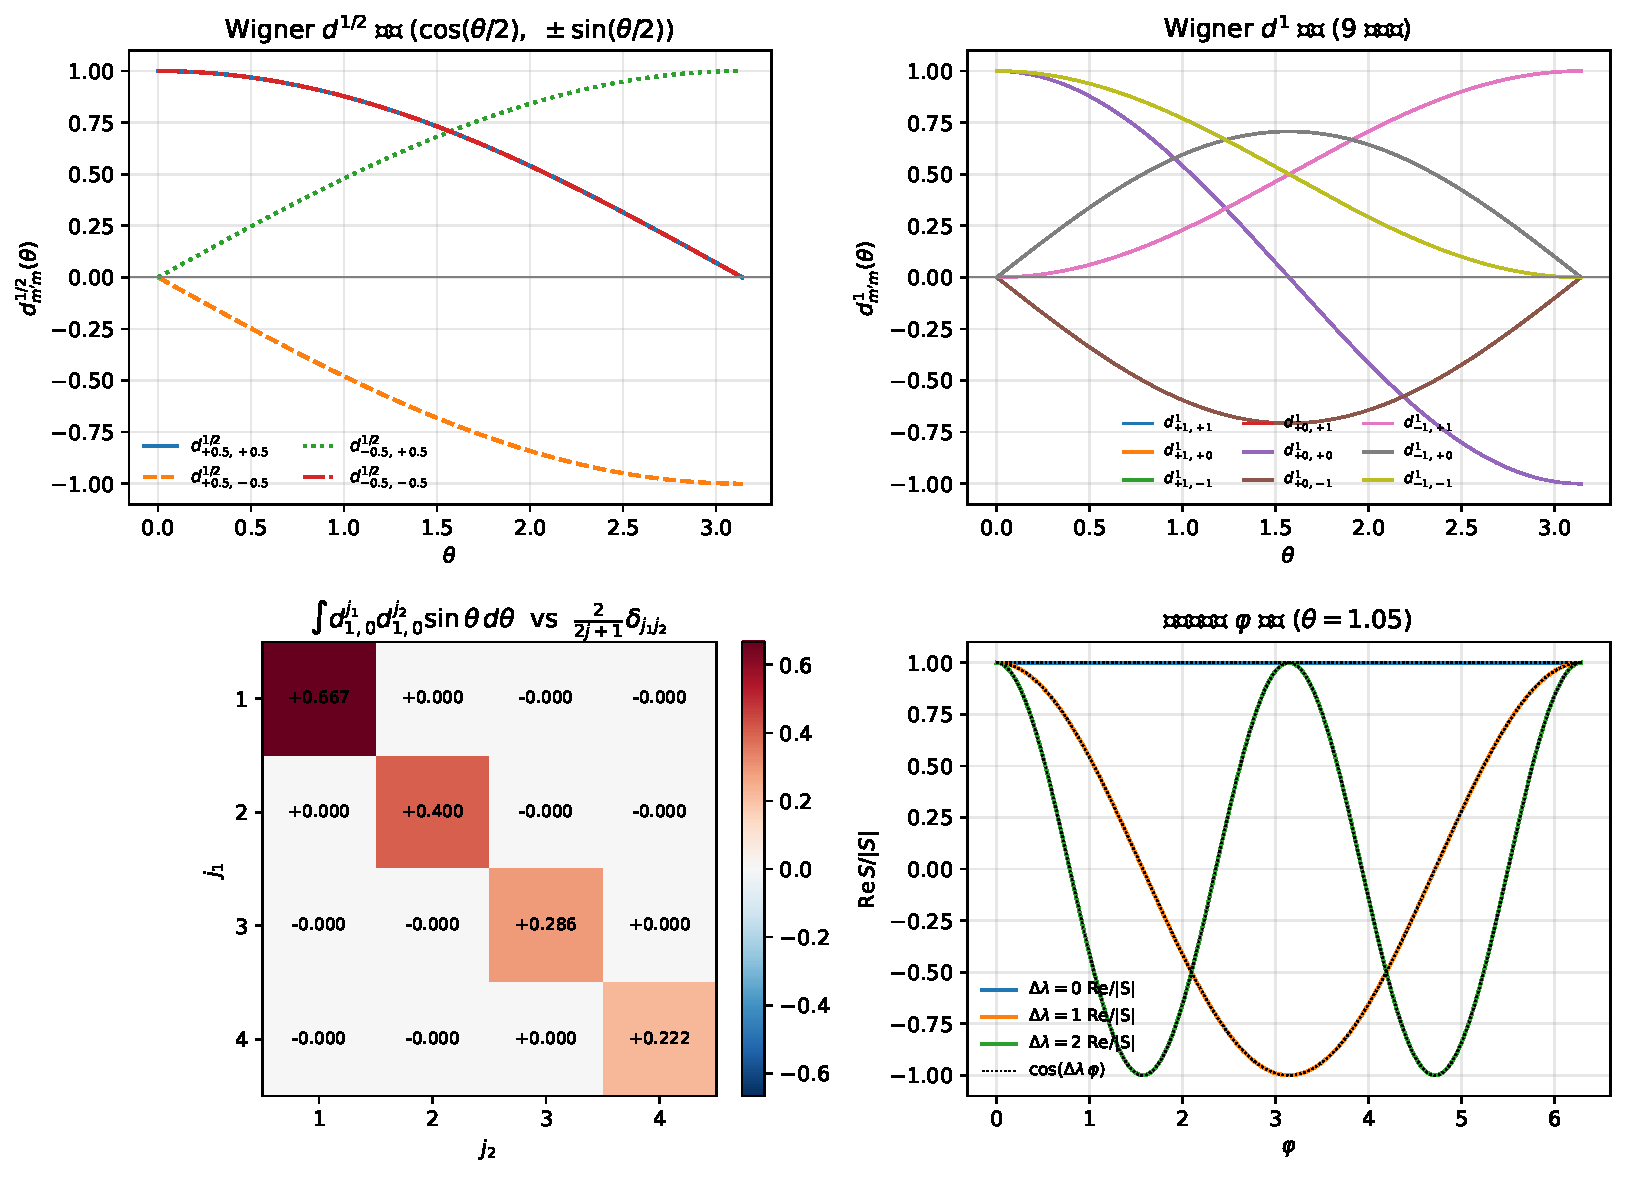
\includegraphics[width=0.95\linewidth]{ch06_wignerD}
    \caption{\textbf{左上}: $d^{1/2}_{m'm}(\theta)$ 的四个分量（解析式 $\pm\cos(\theta/2),\,\pm\sin(\theta/2)$）。\textbf{右上}: $d^{1}_{m'm}(\theta)$ 的九个分量；中心元 $d^1_{00}=\cos\theta$、对角 $d^1_{\pm1,\pm1}=(1\pm\cos\theta)/2$。\textbf{左下}: 在固定 $(m',m)=(1,0)$ 下，对 $j_1,j_2\in\{1,2,3,4\}$ 的内积矩阵热图，仅对角非零、值依次为 $\tfrac{2}{2j+1}=\{2/3,2/5,2/7,2/9\}$，与解析公式偏差 $\sim 2\times 10^{-16}$。\textbf{右下}: 玩具螺度振幅 $\mathrm{Re}\,S/|S|$ 关于方位角 $\varphi$（$\theta=\pi/3$ 固定），三条曲线的相位斜率拟合给出 $\Delta\lambda=0,1,2$，与黑色虚线 $\cos(\Delta\lambda\varphi)$ 完全重合。}
    \label{fig:numexp-ch06}
\end{figure}

\subsection*{物理讨论}
\begin{itemize}
    \item \textbf{$d^{1/2}$ 是 SU(2) 双覆盖的“原子单元”}。所有半整数自旋的小 $d$ 函数都可以通过角动量耦合从 $d^{1/2}$ 得到；$2\pi$ 旋转给出 $-\mathbb{1}$（$d^{1/2}_{m'm}(2\pi)=-\delta_{m'm}$），即旋量的负号特征，是中子干涉实验等的实验基础。
    \item \textbf{$j$-正交性是部分波分解可逆的代数前提}。它使得在螺度基下的展开
    \[
        f_{\lambda_c\lambda_d,\lambda_a\lambda_b}(\theta,\varphi)=\sum_{j}\tfrac{2j+1}{4\pi}\,T^j_{\lambda_c\lambda_d,\lambda_a\lambda_b}\,d^j_{\lambda_a-\lambda_b,\lambda_c-\lambda_d}(\theta)\,\rme^{\rmi(\lambda_a-\lambda_b-\lambda_c+\lambda_d)\varphi}
    \]
    可以唯一反解出分波振幅 $T^j$；数值实验给出的对角值 $2/(2j+1)$ 正是反演公式中的归一化因子。
    \item \textbf{$\varphi$ 因子的物理意义}：旋转 $R_z(\varphi)$ 同时作用于初末态，仅改变螺度本征值的相位，故振幅必呈 $\rme^{\rmi\,\Delta\lambda\varphi}$。这一因子在 (i) 极化截面（截面 $\propto |f|^2$ 时方位依赖只来自不同 $\Delta\lambda$ 干涉项）、(ii) 张量分析力 $T_{20}$（仅 $\theta$ 依赖，例~\ref{eq:morespin-T20-helicity}）、(iii) 单自旋不对称 $A_y\propto\sin\varphi$（仅 $\Delta\lambda$ 奇数项贡献）等观测量中都直接显现。数值拟合得到的相位斜率 $\{0,1,2\}$ 精确等于 $\Delta\lambda$，确证了命题~\ref{prop:morespin-flipphi} 的全部内容。
\end{itemize}
